% Festlegung des allgemeinen Dokumentenformats
\documentclass[a4paper,12pt]{article}

% Schrift
\usepackage[T1]{fontenc}
\usepackage{lmodern}
\usepackage[utf8]{inputenc}
\usepackage[ngerman]{babel}

% Bilder
\usepackage{graphicx}
\usepackage{float}
\graphicspath{{./assets/img}}

% Variablen
% Variablen
\newcommand{\titleDocument}{Bachelorarbeit}
\newcommand{\subjectDocument}{im Studiengang Informatik}
\newcommand*{\bildquelle}{
  \footnotesize Quelle:
}
\newcommand{\code}[1]{\noindent\ignorespaces\texttt{#1}}

% Code
\usepackage{listings}
\usepackage{color}

\definecolor{black}{rgb}{0,0,0}
\definecolor{dkgreen}{rgb}{0,0.6,0}
\definecolor{gray}{rgb}{0.5,0.5,0.5}
\definecolor{mauve}{rgb}{0.58,0,0.82}

\lstset{literate=%
    {Ö}{{\"O}}1
    {Ä}{{\"A}}1
    {Ü}{{\"U}}1
    {ß}{{\ss}}1
    {ü}{{\"u}}1
    {ä}{{\"a}}1
    {ö}{{\"o}}1
    {~}{{\textasciitilde}}1
}

\lstdefinestyle{Bash} {
  frame=single,
  language=Bash,
  aboveskip=3mm,
  belowskip=3mm,
  showstringspaces=false,
  columns=flexible,
  basicstyle={\small\ttfamily},
  numbers=none,
  numberstyle=\tiny\color{black},
  keywordstyle=\color{black},
  commentstyle=\color{black},
  stringstyle=\color{black},
  breaklines=true,
  breakatwhitespace=true,
  tabsize=3
}

\lstset{emph={\$},emphstyle=\textbf}

\lstdefinestyle{Python} {
  frame=single,
  language=Bash,
  aboveskip=3mm,
  belowskip=3mm,
  showstringspaces=false,
  columns=flexible,
  basicstyle={\small\ttfamily},
  numbers=left,
  numberstyle=\tiny\color{black},
  keywordstyle=\color{black},
  commentstyle=\color{gray},
  stringstyle=\color{gray},
  breaklines=true,
  breakatwhitespace=true,
  tabsize=2
}

% mehrseitige Tabellen ermöglichen
\usepackage{longtable}
\usepackage{diagbox}

% Packet für Seitenrandabstände und Einstellung für Seitenränder
\usepackage{geometry}
\geometry{left=3.5cm, right=2.5cm, top=2.5cm, bottom=2cm}

% bricht lange URLs "schön" um
\usepackage[hyphens,obeyspaces,spaces]{url}

% Festlegung Art der Zitierung
\usepackage{csquotes}
\usepackage[style=apa, backend=biber]{biblatex}
\addbibresource{assets/literatur.bib}

% Abstand zwischen Absätze
\setlength{\parindent}{2em}
\setlength{\parskip}{1em}

% Paket für Zeilenabstand
\usepackage[onehalfspacing]{setspace}

% für Bildbezeichner
\usepackage{capt-of}

% für Stichwortverzeichnis
\usepackage{makeidx}

% für Abkürzungsverzeichnis
\usepackage{acronym}

% Für Phantomsection
\usepackage{hyperref}

% Für Tabellen
\usepackage{tabularx}

% Konfiguriere das Inhaltsverzeichnis
\usepackage{tocbasic}

% \DeclareTOCStyleEntries[
%   raggedentrytext,
%   numwidth=0pt,
%   numsep=1ex,
%   dynnumwidth,
% ]{tocline}{chapter,section,subsection,subsubsection,paragraph,subparagraph}
% \DeclareTOCStyleEntries[
%   indent=0pt,
%   linefill=\TOCLineLeaderFill,
% ]{tocline}{section,subsection,subsubsection,paragraph,subparagraph}

% subsubsubsection durch paragraph
\usepackage{titlesec}
\setcounter{secnumdepth}{4}
\titleformat{\paragraph}
{\normalfont\normalsize\bfseries}{\theparagraph}{1em}{}
\titlespacing*{\paragraph}
{0pt}{3.25ex plus 1ex minus .2ex}{1.5ex plus .2ex}

% Titel
\title{Bachelorarbeit}

% Autor
\author{Andreas Huber}

% Datum
\date{\today}

%
% Start
% des
% Dokuments
%
\begin{document}

% Titelseite
\thispagestyle{empty}

\begin{figure}[t]
 \centering
 
\includegraphics[width=0.4\textwidth]{assets/oth/logo}
\end{figure}

\begin{verbatim}
\end{verbatim}

\begin{center}
    \Large{Ostbayerische Technische Hochschule Regensburg} \\
    \Large{Fakultät für Informatik und Mathematik}
\end{center}

\begin{verbatim}
\end{verbatim}

\begin{center}
    \doublespacing
    \textbf{\huge{\titleDocument}}\\

    \onehalfspacing

    \begin{center}
        Zur Erlangung des akademischen Grades \\ Bachelor of Science (B. Sc.)
    \end{center}

    \begin{verbatim}
    \end{verbatim}

    \begin{doublespace}
        \textbf{\Large{{~\subjectDocument}}}
    \end{doublespace}
\end{center}

\begin{verbatim}
\end{verbatim}

\begin{verbatim}
\end{verbatim}

\begin{flushleft}
    \begin{tabularx}{\linewidth}{@{}>{\bfseries}l@{\hspace{.9em}}X@{}}
        \textbf{Vorgelegt von:} & Andreas Huber <andreas.huber@st.oth-regensburg.de> \\
        \textbf{Matrikelnummer:}& 3180161 \\
        \textbf{Studiengang:}   & Allgemeine Informatik \\
                                & \\
        \textbf{Erstgutachter:} & Prof. Dr. Markus Heckner \\
        \textbf{Zweitgutachter:}& Prof. Dr. Johannes Schildgen \\
                                & \\
        \textbf{Abgabefrist:}   & 25. April 2022 \\
    \end{tabularx}
\end{flushleft}
\newpage

% Römische Nummerierung
\pagenumbering{roman}

% Inhaltsverzeichnis
\tableofcontents
\newpage

% Abkürzungsverzeichnis
\phantomsection
\section*{Abkürzungsverzeichnis}
\addcontentsline{toc}{section}{Abkürzungsverzeichnis}

\begin{acronym}[Bash]
    \acro{bash}[Bash]{Bourne-again shell}
    \acro{ide}[IDE]{Integrated Development Environment}
    \acro{ldap}[LDAP]{Lightweight Directory Access Protocol}
    \acro{lms}[LMS]{Learning Management System}
    \acro{oth}[OTH]{Ostbayerische Technische Hochschule}
    \acro{sd}[SD]{Standardabweichung}
\end{acronym}
\newpage

% Arabische Seitennummerierung ab hier
\pagenumbering{arabic}

% Einleitung
\section{Einleitung und Motivation}\label{einleitung}
\subsection{Herausforderung digitales Lernen}\label{herausforderung}
Deutschland gilt als sehr rückschrittlich im Thema Digitalisierung an Schulen
und Universitäten. Nicht zuletzt hat die Corona-Pandemie viele
Bildungseinrichtungen dazu gezwungen, umzudenken und digitale Lerninhalte
zu erstellen. Mit dieser Herausforderung kamen jedoch einige Einrichtungen und
Lehrende schnell an ihre Grenzen. Die Hochschule Regensburg hat ein optionales
Zusatzsstudium entwickelt, um die sogenannten \glqq Digital Skills\grqq{}
der Studierenden zu verbessern und zu intensivieren. 

\subsection{Kurs Digital Skills als Zusatzstudium}\label{kurs-digital-skills}
Digital Skills ist ein aus drei Semester bestehendes Zusatzstudium für alle
Studierenden, mit Ausnahme von Studierenden der Fakultät Informatik und
Mathematik, der Hochschule Regensburg. Das Zusatzstudium soll den Teilnehmern
vor allem digitales Wissen näher bringen. In Semester 1 lernen die Studierenden
unter dem Motto \glqq Technologische Skills\grqq{} die Grundlagen der
Programmierung, sowie das Verständnis von Internet of Things. Das zweite
Semester befasst sich mit \glqq Future Work Skills\grqq{} und bringt den
Teilnehmern das Verständnis der Themen Data Science, Digitale Ethike,
Agile Working, sowie Coaching Fähigkeiten bei. Im letzten Semester haben die
Lernenden die Möglichkeit ein eigenes Digitalisierungsprojekt zu planen und
umzusetzen.

Um im ersten Semester die Grundlagen der Programmierung automatisiert und
trotzdem mit Feedback zu lehren, wird eine zeit- und ortsunabhängige innovative
Lernplattform benötigt. Genau mit dieser Aufgabe beschäftigt sich der Kern
dieser Arbeit.

\subsection{Struktur der Arbeit}\label{struktur-der-arbeit}
Die Arbeit besteht aus mehreren wesentlichen Bestandteilen. Kapitel
\ref{anforderungsanalyse} behandelt alle nötigen Anforderungen, die für den
Aufbau einer digitalen Lernplattform wichtig sind. Kapitel
\ref{softwarearchitektur} wiederum vergleicht und diskutiert zuerst vorhandene
Lern-Systeme und trifft dann die finale Entscheidung für den Kurs Digital
Skills. Die finale Entscheidung und deren Konfiguration und Implementierung wird
dann folgend in Kapitel \ref{konfiguration-u-impl} näher erläutert und
beschrieben. Schließlich wird die Programmierlernplattform in Kapitel
\ref{studie} in Form einer kleinen Studie an nicht Informatik- oder Mathematik-
studierenden Testprobanden getestet. Schließlich fasst Kapitel
\ref{zusammenfassung-u-ausblick} alles zusammen und gibt einen weiteren Ausblick
auf die Zukunft des Systems.

% Anforderungsanalyse
\newpage
\section{Anforderungsanalyse}\label{anforderungsanalyse}
Funktionale Anforderungen beschreiben, welche Features und Funktionen das
Projekt bieten muss. Diese Informationen sind wichtig, um die richtigen
Werkzeuge und Programme für die Umsetzung auszuwählen. Dabei geht es meist um
sehr konkret formulierte Wünsche. Nichtfunktionale Bedingungen sind wiederum
Bedingungen, wie zum Beispiel Zuverlässigkeit, Verfügbarkeit oder diverse
Sicherheitsanforderungen. Sie lassen sich eher als Qualitätseigenschaften
beschreiben.

Die folgenden Anforderungen werden durch die wissenschaftliche Mitarbeiterin
Julia Ruhland und dem Studierenden Andreas Huber festgelegt. Die funktionalen
Anforderungen werden durch Andreas Huber aufgestellt und in wöchentlichen
Meetings mit Prof. Dr. Heckner verifiziert. Andreas Huber sammelt außerdem
gemeinsam mit Julia Ruhland User-Stories aus der Sicht der Studierenden und den
Dozierenden in der Online-Plattform Trello. Die nichtfunktionalen Anforderungen
werden wiederum von den User-Stories abgeleitet. % TODO: Anhang

\subsection{Funktionale Anforderungen}\label{anforderungsanalyse-funktional}
\subsubsection{Studierende}\label{anforderungsanalyse-funktional-stud}
Den Studierenden sollte eine Kursübersicht mit allen Aufgaben zur Verfügung
gestellt werden. Der persönliche Fortschritt der jeweiligen Aufgaben sollte
dabei leicht ersichtlich sein. Mögliche Deadlines oder Abgabefristen sollen bei
jeder Aufgabe deutlich erkennbar sein.

Des Weiteren muss es Studierenden möglich sein, ohne die Installation von
zusätzlichen Programmen, die Aufgaben online bearbeiten, prüfen und abgeben zu
können. Trotzdem sollen ihnen die Option offen stehen, die Übungen in der
Entwicklungsumgebung ihrer Wahl lösen zu können.

Eine weitere wichtige Anforderung bei der Prüfung der Aufgaben ist, dass die
Bearbeiter der Aufgaben sogenannte \emph{human-readable} (für den Menschen
lesbare) Fehlermeldungen erhalten müssen. Das bedeutet, dass die Fehlermeldungen
bei der Überprüfung auch für fachfremde Studierende leicht verständlich sein
müssen. Fehlermeldungen bzw. konstruktives Feedback muss dabei automatisiert und
jederzeit generiert werden können.

Die Möglichkeit, Aufgabenversuche abzugeben, muss ebenfalls mit wenig Aufwand
behaftet sein. Falls ein Versuch fehlschlägt, oder nicht die volle Punktzahl
erreicht wird, sollte der Teilnehmende jederzeit die Möglichkeit haben, einen
neuen Versuch hochladen zu können.

\subsubsection{Lehrende}\label{anforderungsanalyse-funktional-lehrende}
Lehrende müssen neue Aufgaben anlegen und konfigurieren können, dazu gehört
unter anderem die Festlegung eines Abgabedatums.

Zusätzlich müssen Dozierende die Möglichkeit haben eine Übersicht an Aufgaben
des jeweiligen Kurses einzusehen und davon einzelne Übungen temporär zu
verstecken oder zu deaktivieren.

Darüber hinaus muss es möglich sein, mehrere Administratoren zu den Kursen
hinzuzufügen. Dadurch können verschiedene Personen Aufgaben erstellen und die
abgegebenen Lösungen herunterladen. Dies ist gleichzeitig die nächste
Anforderung: Administratoren müssen mit wenig Aufwand alle Abgaben der
Teilnehmenden herunterladen können.

Ferner müssen sowohl die Aufgaben, als auch die jeweiligen Deadlines nach der
Erstellung editierbar sein. Dadurch können Dozierende ihre Aufgaben stetig
verbessern.

Um einen Überblick über den Schwierigkeitsgrad der Aufgaben behalten zu können,
müssen Lehrende den Aufgaben-Fortschritt der Studierenden je nach Kurs
übersichtlich einsehen können. Sollte ein Großteil der Teilnehmenden an
einzelnen Aufgaben scheitern, kann die Aufgabenstellung im Einzelnen erneut
evaluiert und verbessert werden.

\subsection{Nichtfunktionale Anforderungen}
\label{anforderungsanalyse-nichtfunktional}
Das eingesetzte System muss neben den funktionalen Anforderungen auch diverse
nichtfunktionale Anforderungen erfüllen, um von der OTH als sinnvolle
Lernplattform eingesetzt werden zu können.

Der erste wichtige Punkt ist, dass die Lernplattform möglichst zuverlässig ist.
Zur Zuverlässigkeit gehört neben einer hohen Verfügbarkeit auch eine skalierende
Performance, wenn viele Studierende gleichzeitig die Software nutzen wollen.

Ein weiterer Punkt ist die Wartbarkeit. Die Plattform sollte mit möglichst wenig
Wartung sicher bestehen bleiben können. Außerdem sollte nur auf externe Systeme
gesetzt werden, von denen ausgegangen werden kann, dass diese noch einige Jahre
gepflegt werden. Hier empfiehlt sich ein Aufteilen der Plattform auf mehrere
externe Tools, um bei einem Ausfall oder Außerbetriebnahme eines einzelnen Tools
noch einen Notbetrieb gewährleisten zu können. Der Austausch gegen eine andere
neue Softwarekomponente gestaltet sich dadurch leichter.

Die Ressourcenlast und die damit verbundenen Kosten spielen eine weitere
wichtige Rolle bei der Entscheidungsfindung. Wenn Teile der Lernplattform auf
OTH-Servern gehostet werden müssen, sollten diese möglichst ressourcenschonend
sein. Serverressourcen sind teuer und können das Projekt im Zweifelsfall
unrentabel machen, wenn das System bei paralleler Nutzung durch mehrere
Studierende eine inadäquate Serverlast voraussetzen würde. Selbiges gilt für
Lizenzgebühren möglicher Tools und Werkzeuge.

Neben den Kosten ist es auch wichtig, dass die Plattform zusammen mit dem
\ac{lms} bzw. der Lernplattform der Hochschule arbeiten kann. Der Vorteil einer
LMS-Integration wird später im \autoref{code-freak} näher erläutert.

Zu guter Letzt ist es wünschenswert, dass der Programmierkurs bei der Auswahl
der Programmiersprache flexibel ist. So sollte es beispielsweise möglich sein,
dass die erste Aufgabe mit der Programmiersprache Java gelöst wird,
während die zweite mit Python gelöst werden muss.

% Softwarearchitektur
\newpage
\section{Softwarearchitektur}
Dieses Kapitel befasst sich mit der für das Projekt benötigten Toolchain.
Eine Toolchain ist eine Sammlung verschiedener Anwendungen, die gemeinsam eine
Lösung bzw. ein Produkt erzeugen. Durch den Vergleich mit verschiedenen
bestehenden digitalen Lernplattformen ist es möglich, optimale 
Software-Werkzeuge für die Hochschule Regensburg zu finden und schließlich
einzusetzen.

% Vergleich vorhandener Systeme
\subsection{Vergleich vorhandener Systeme}
\subsubsection{CS50 der Harvard University}
\paragraph{Allgemeines}
CS50 ist die ursprüngliche Bezeichnung eines Lernkurses über Informatik,
welcher von der Harvard University ins Leben gerufen wurde und weiterhin
betreut wird. Der Kurs wurde aufgrund seines Erfolgs digitalisiert und wird nun
als CS50x auf der Lernplattform edX angeboten. Folgende Recherchen und Aussagen
sind jeweils immer auf die Online-Version CS50x bezogen.

Der Kurs CS50 lehrt Schüler\footnote{Aus Gründen der besseren Lesbarkeit wird
in der gesamten Arbeit auf die gleichzeitige Verwendung der Sprachformen
männlich, weiblich und divers (m/w/d) verzichtet. Sämtliche
Personenbezeichnungen gelten gleichermaßen für alle Geschlechter. Ist eine
spezifische Geschlechtergruppe gemeint, wird das entsprechende Adjektiv
vorangestellt (z.B. \glqq männliche Studenten\grqq)} die Grundlagen der
Informatik. Dabei werden diverse Programmierübungen abgefragt. Aufgrund der
hohen Anzahl an Teilnehmern besitzt der Kurs ein automatisiertes Abgabe- und Benotungssystem.

Das System hinter CS50 wird mittlerweile vielfältig eingesetzt und wurde zu
einem universalen Online-Lernsystem erweitert. Jeder kann sich durch eine
Authentifizierung über die Plattform GitHub im Abgabesystem von CS50 einloggen
und eigene Kurse erstellen. \cite{cs50}

\newpage
\paragraph{Ablauf für Studierende}
Dem Teilnehmer wird jede Woche ein neues Kapitel präsentiert. Er kann sich dabei
sowohl durch ein Vorlesungsvideo, als auch durch geschriebene Materialien über
das Thema der Woche informieren. Mit Beginn der Woche bekommt der Teilnehmer
neben den Materialien auch Programmieraufgaben, welche er mit dem vorher
genannten System bearbeiten kann. \cite{cs50-edx}

Die Programmieraufgaben können wahlweise über die, auf AWS Cloud9 basierenden,
Online-Entwicklungsumgebung \glqq CS50-IDE\grqq{} von Harvard oder in jeder
anderen beliebigen Entwicklungsumgebung der Wahl bearbeitet werden. Dies
wird durch die Architektur des Systems ermöglicht. Jede Funktionalität der
Automatisierung geschieht durch Kommandozeilen-Tools. Dieses System hat den
Vorteil, dass es unabhängig von der eingesetzten IDE funktioniert, es wird
lediglich ein Terminal mit den jeweiligen Tools benötigt. \cite{cs50-ide}

Vor der Abgabe der endgültigen Lösung mit dem sogenannten Werkzeug
\glqq submit50\grqq{}, ist es möglich den Code mit einem weiteren Werkzeug
namens \glqq check50\grqq{} überprüfen zu lassen. Außerdem gibt es viele weitere
Werkzeuge, ein Beispiel hierfür ist \glqq style50\grqq{}, welches die Qualität
und den Style des Programmcodes überprüft und bewertet. \cite{submit50}

\paragraph{Architektur}
Die Harvard University hält den Aufbau von CS50 weitestgehend transparent.
Viele der eingesetzten Werkzeuge sind öffentlich als Open-Source-Projekte unter
der GitHub-Organisation \glqq CS50\grqq{} zu finden \cite{cs50-github}. Darunter
befinden sich unter Anderem folgende Projekte:
\begin{itemize}
\item submit50: Abgabe von Code
\item check50: Funktionalitätstests des Codes
\item render50: Erzeugung von .PDF-Dateien aus Code
\item ide50: Online-Entwicklungsumgebung
\item style50: Überprüfung der Code-Qualität
\item compare50: Plagiatserkennung von abgegebenen Projekten
\item server50: Webserver
\end{itemize}

\newpage

In Abbildung \ref{fig:cs50-architektur} ist der Aufbau der Lernplattform CS50
vereinfacht grafisch dargestellt. Die Rechtecke und Menschen sind die
beteiligten Komponenten. Die Pfeile zwischen den Komponenten beschreiben die
verbindende Relation. Die von der \glqq CS50-Programm\grqq-Komponente
ausgehenden gestrichelten Pfeile zeigen, je nach ausgeführtem Befehl,
mögliche Relationen.

\begin{figure}[h]
    \centering
    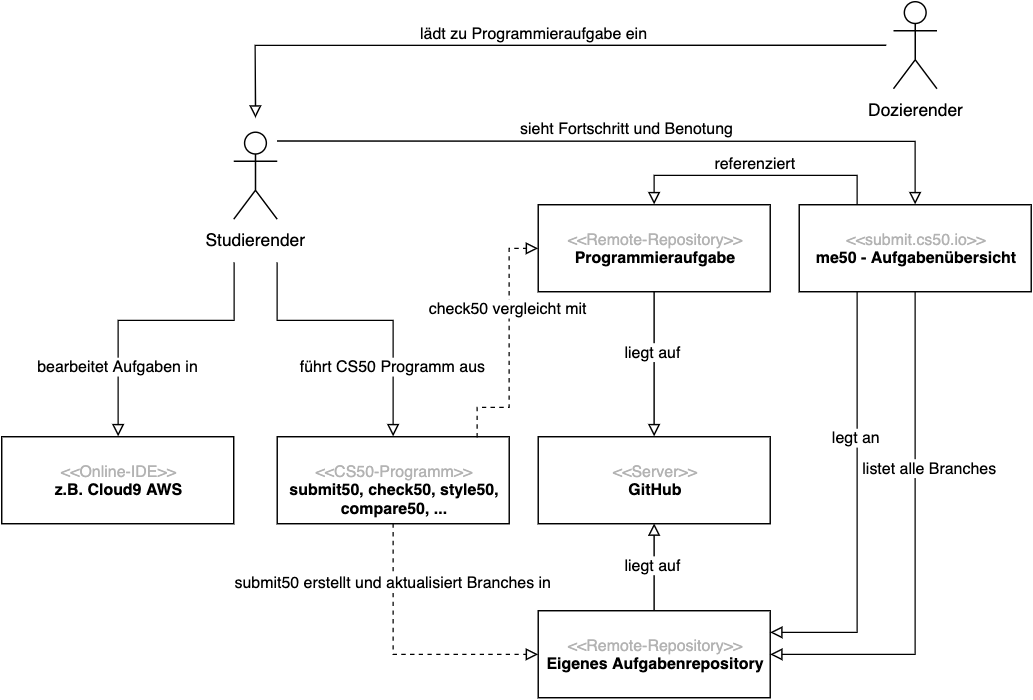
\includegraphics[width=\textwidth]{cs50-architektur}
    \caption{CS50 Architektur}
    \bildquelle{Eigene Darstellung}
    \label{fig:cs50-architektur}
\end{figure}

\paragraph{Probleme beim Einsatz für die OTH}
Die Toolchain von CS50 wäre adäquat für den Einsatz an der OTH-Regensburg.
Eines der Projekte ist aktuell noch nicht Open-Source: Die Website zur
Erstellung von neuen Kursen, Abgaben und Mitgliederverwaltung. Dieses Projekt
ist essentiell für die Verwendung der Werkzeuge an der Regensburger Hochschule.
Nach Rücksprache mit Herr X der Harvard University ist ein Neuaufbau dieser
Website mit einhergehender Veröffentlichung als Open-Source-Projekt gerade in
Planung. Einen genauen öffentlichen Zeitplan hierfür gibt es aktuell nicht. In
Folge dessen ist ein Einsatz des CS50-Systems an der OTH zum heutigen Datum
nicht möglich.

\newpage
\subsubsection{Code FREAK der Fachhochschule Kiel}
\paragraph{Allgemeines}
Code FREAK ist eine All-In-One Lösung für Online-Programmieraufgaben mit
automatisiertem Feedback. Die von der Hochschule Kiel entwickelte Open-Source
Software soll den Einstieg in eine digitale Lernumgebung einfach machen. Die
Zielgruppe von Code FREAK bezieht sich hierbei explizit auf Universitäten und
Einrichtungen einer höheren Bildung. \cite{codefreak-startseite}

Desweiteren wirbt Code FREAK mit einer LMS-Integration. LMS ist die englische
Abkürzung für Learning Management System (dt. Lernplattform). Viele Schulen und
Universitäten verwendenx bekannte LMS-Systeme, wie Moodle, um Kurse, Fächer und
Studierende zu verwalten. \cite{moodle}
Dies hat den Vorteil, dass Studierende kein extra Nutzerkonto für Code FREAK
anlegen müssen. Sie können sich direkt mit ihrem gewohnten Zugang anmelden.

\paragraph{Ablauf für Studierende}
Studierende können nach Anmeldung am System, an für sie sichtbaren Kursen
(Assignments) teilnehmen. Dies geschieht meist durch einen vom Dozenten
generierten Einladungslink. Jedes Assignment kann mehrere Aufgaben (Tasks)
enthalten. Die einzelnen Aufgaben können dann entweder über die integrierte
Online-Entwicklungsumgebung, durch Hochladen der Lösung, oder durch die Angabe
eines Git-Repository-Links bearbeitet werden.

Mit dem Klick auf den Knopf \glqq Start Evaluation\grqq{} wird hochgeladene
Lösung der Aufgabe überprüft. Die Ergebnisse der einzelnen Test-Schritte können
dann in einem weiteren Tab eingesehen werden. Wenn alle Tests der Aufgabe
bestanden wurden, wird der Task mit einem grünen Haken versehen. So sieht der
Schüler in der Assignment-Ansicht auf einen Blick, welche Aufgaben er bereits
gelöst hat.

\paragraph{Architektur}
Code FREAK wird als fertiger Docker-Container ausgeliefert. Docker ist eine
Software um mit Hilfe von Containervirtualisierung einzelne Anwendungen
voneinander zu isolieren. Durch die Containervirtualisierung werden unter
Anderem viele Abhängigkeits- und Deploymentprobleme beseitigt. Der Container
enthält alle Bibliotheken und Abhängigkeiten, die die Software für die Laufzeit
benötigt \cite{docker}. Docker entstand auf Basis von Linux-Containern, welche
ein oder mehrere Prozesse vom restlichen System isolieren können 
\cite{linux-container}.

Durch diese Handhabung, kann Code FREAK mit nur einem Befehl in der
Kommandozeile installiert und gestartet werden. Die Software benötigt
grundsätzlich nur einen Container. Benutzt ein Studierender jedoch die
integrierte Online-Entwicklungsumgebung (Online-IDE), muss für jede Instanz ein
zusätzlicher Container mit der Laufzeitumgebung der IDE gestartet werden. Jeder
weitere Container benötigt weiteren Arbeitsspeicher.

\paragraph{Probleme beim Einsatz für die OTH}
Beim Einsatz von Code FREAK an der Hochschule Regensburg gibt es einige
Probleme. Das erste Problem bezieht sich auf den vorher erwähnten
Arbeitsspeicher. Die Praxis zeigt, dass eine Instanz der Online-IDE schon nach
wenigen Dateien ~3 Gigabytes an Arbeitsspeicher verwendet. Um eine reibungslose
und parallele Nutzung für alle Studierende des Kurses gewährleisten zu können,
werden dementsprechend sehr hohe Serverkosten fällig. 
\cite{codefreak-memory-problem}

Ein weitere Hürde ist die Stabilität der Software. Code FREAK befindet sich,
Stand heute, mitten in der Entwicklung, weshalb einige Funktionen und Features
noch nicht ordnungsgemäß funktionieren. Darunter die vorher geworbene
LMS-Integration. \cite{codefreak-docs} Zum heutigen Zeitpunkt ist LDAP die
einzige Möglichkeit sich mit dem System zu authentifizieren. Ein eigenes Anmeldeverfahren gibt es nicht.

LDAP steht für Lightweight Directory Access Protocol und ist ein
Netzwerkprotokoll zur Durchführung von Abfragen und Änderungen in einem 
verteilten Verzeichnisdienst. LDAP ist der De-facto Industriestandard für
Authentifizierung und Autorisierung. \cite{ldap}

Der Kurs Digital Skills soll den Teilnehmern einen Überblick über den
Arbeitsalltag eines Informatikers geben. Dazu gehört unter anderem die
Kommandozeile. Eine Anforderung der Lernplattform ist deshalb, dass man
(optional) neue Aufgaben herunterladen und Lösungsversuche über Befehle in der
Kommandozeile testen und abgeben kann. In Code FREAK kann man Aufgaben lediglich
über die Oberfläche testen und abgeben.

\newpage
\subsubsection{GitHub Classroom}
\paragraph{Allgemeines}
GitHub Classroom ist ein weiterer Kandidat für den Einsatz an der
Hochschule Regensburg. Die Plattform ermöglicht die automatisierte
Erstellung von Repositories auf GitHub. Außerdem hilft Classroom dabei,
Aufgabenvorlagen und dazugehörige Abgaben einfach zu verwalten und automatisch
zu benoten. Dabei enthalten die von GitHub Classroom erstellten
Aufgaben-Repositories bereits vorkonfigurierte Zugriffskontrollen. \cite{github-classroom-startseite}

\paragraph{Ablauf für Studierende}
Studierende bekommen pro Programmieraufgabe einen Einladungslink.
Nach Annahme der Einladung, wird pro Studierenden automatisch ein Repository für
die jeweilige Aufgabe angelegt. Dieses Repository enthält die Vorlage,
welche zum Bearbeiten der Aufgabe benötigt wird.

Sobald der Studierende eine Lösung zur Korrektur abgeben möchte, kann er per
Push die Änderungen in das Remote-Repository hochladen. Je nach Konfiguration
der Aufgabe starten daraufhin serverseitig ein oder mehrere Tests. Wenn alle
Tests bestanden sind, hat der Studierende die Aufgabe erfolgreich abgeschlossen.

\paragraph{Architektur} % TODO: Zitieren?
GitHub Classroom ist ein Bildungsservice der Firma GitHub Inc. und ist Stand
heute kostenfrei \cite{github-classroom-kostenlos}. Die Software basiert auf der Automatisierung von Repositories. Jeder bei GitHub registrierte Nutzer, kann
einen sogenannten \glqq Classroom\grqq erstellen und darin Aufgaben auf Basis
vorhandener öffentlichen GitHub-Repositories erstellen.

\paragraph{Probleme beim Einsatz für die OTH}
Es gibt keine Möglichkeit das System von GitHub Classroom auf einen lokalen
Git-Server zu replizieren. Auf Grund dessen schafft man sich durch die
Verwendung von Classroom eine externe Abhängigkeit an GitHub. Dies kann unter
Umständen zu erheblichen Problemen führen, wenn der Dienst beispielsweise
nicht erreichbar oder aufgelöst wird. Ersteres ist durch die Größe und
Infrastruktur des Unternehmens nicht (häufig) zu erwarten.

Ein weitere Hürde ist der Bedarf an weiterer Software. GitHub Classroom alleine
ist nicht ausreichend, um als vollständige Lernplattform für den Kurs Digital
Skills geeignet zu sein. Hier bietet es sich an, eine eigene statische Website
mit Anleitungen und Erklärungen zu bauen, welche dann jeweils auf Classroom
Einladungslinks verweist. Als Online-Entwicklungsumgebung kann der Dienst Replit
verwendet werden. In Replit ist es möglich, ein vorhandenes Git-Repository als
Template für eine neue Umgebung zu verwenden. Dieses Template könnte
Wrapper-Programme für den git-Workflow enthalten. Der Vorteil daran:
Studierende bekommen erste Erfahrungen mit der Kommandozeile, müssen jedoch
keine komplexen Git-Kommandos absetzen.


% Finale Architektur Online-Learning Platform
\subsection{Finale Architektur Online-Learning Platform}
\subsubsection{Tutors als Aufgabensammlung}
Das freie Open-Source-Projekt Tutors ist eine Sammlung von Softwarepaketen,
die entwickelt wurden, um Online-Kurse mit Vorlesungen, Übungen, Videos und
Kursmaterialien zu erstellen und durchzuführen. \parencite{tutors}

Durch die Funktionalität Kursmaterialien und Übungen zu erstellen, dient Tutors
ideal als Aufgabensammlung des Programmierkurses. Auf der Plattform kann neben
dem Programmierkurs auch der gesamte Inhalt des Zusatzstudiums eingeteilt in
Semester, Module und Labs hochgeladen werden. Im Programmierkursmodul verlinkt
jede Aufgabe jeweils auf den Einladungslink der GitHub-Classroom-Aufgabe.

Neue Anleitungsseiten können mithilfe der in Informatik üblichen
Dokumentensprache Markdown angelegt, formatiert und präsentiert werden. Wie in
Abbildung \ref{fig:markdown} zu sehen, kann eine Markdown-Anleitung in jedem
beliebigen Text-Editor geschrieben werden.

In diesem Fall befindet sich links der Text-Editor und rechts die Vorschau des
daraus interpretierbaren Dokuments. Grundsätzlich bleibt eine Markdown-Datei
unkompiliert, das heißt die geschriebene Textdatei ist alles was man für das
Dokument benötigt. Es gibt jedoch einige Programme und Tools, die die Dateien
nach einem gewissen Standard interpretieren.

Zeile 11 des Markdown-Dokuments in Abbildung \ref{fig:markdown} zeigt eine
Überschrift, welche durch zwei Rautezeichen (\code{\#\#}) markiert wird. Diese
Überschrift ist bereits eine Unterüberschrift. Der Titelüberschrift wird
lediglich ein Rautezeichen vorangesetzt, währenddessen eine
Unterunterüberschrift drei Rautezeichen benötigt (siehe Zeile 29 in Abbildung
\ref{fig:markdown}).

Projekte, wie Tutors, interpretieren diese Rautezeichen als Überschrift und
können so die Schriftgröße und Abstände für alle hinter den Rautezeichen
stehenden Wörter anpassen. Das Rautezeichen ist nur ein Beispiel für eines von
vielen verschiedenen Formatierungszeichen. Aus diesen simplen
Formatierungszeichen entsteht später für den Teilnehmenden ein gut lesbares
Online-Dokument.

\begin{figure}[H]
    \centering
    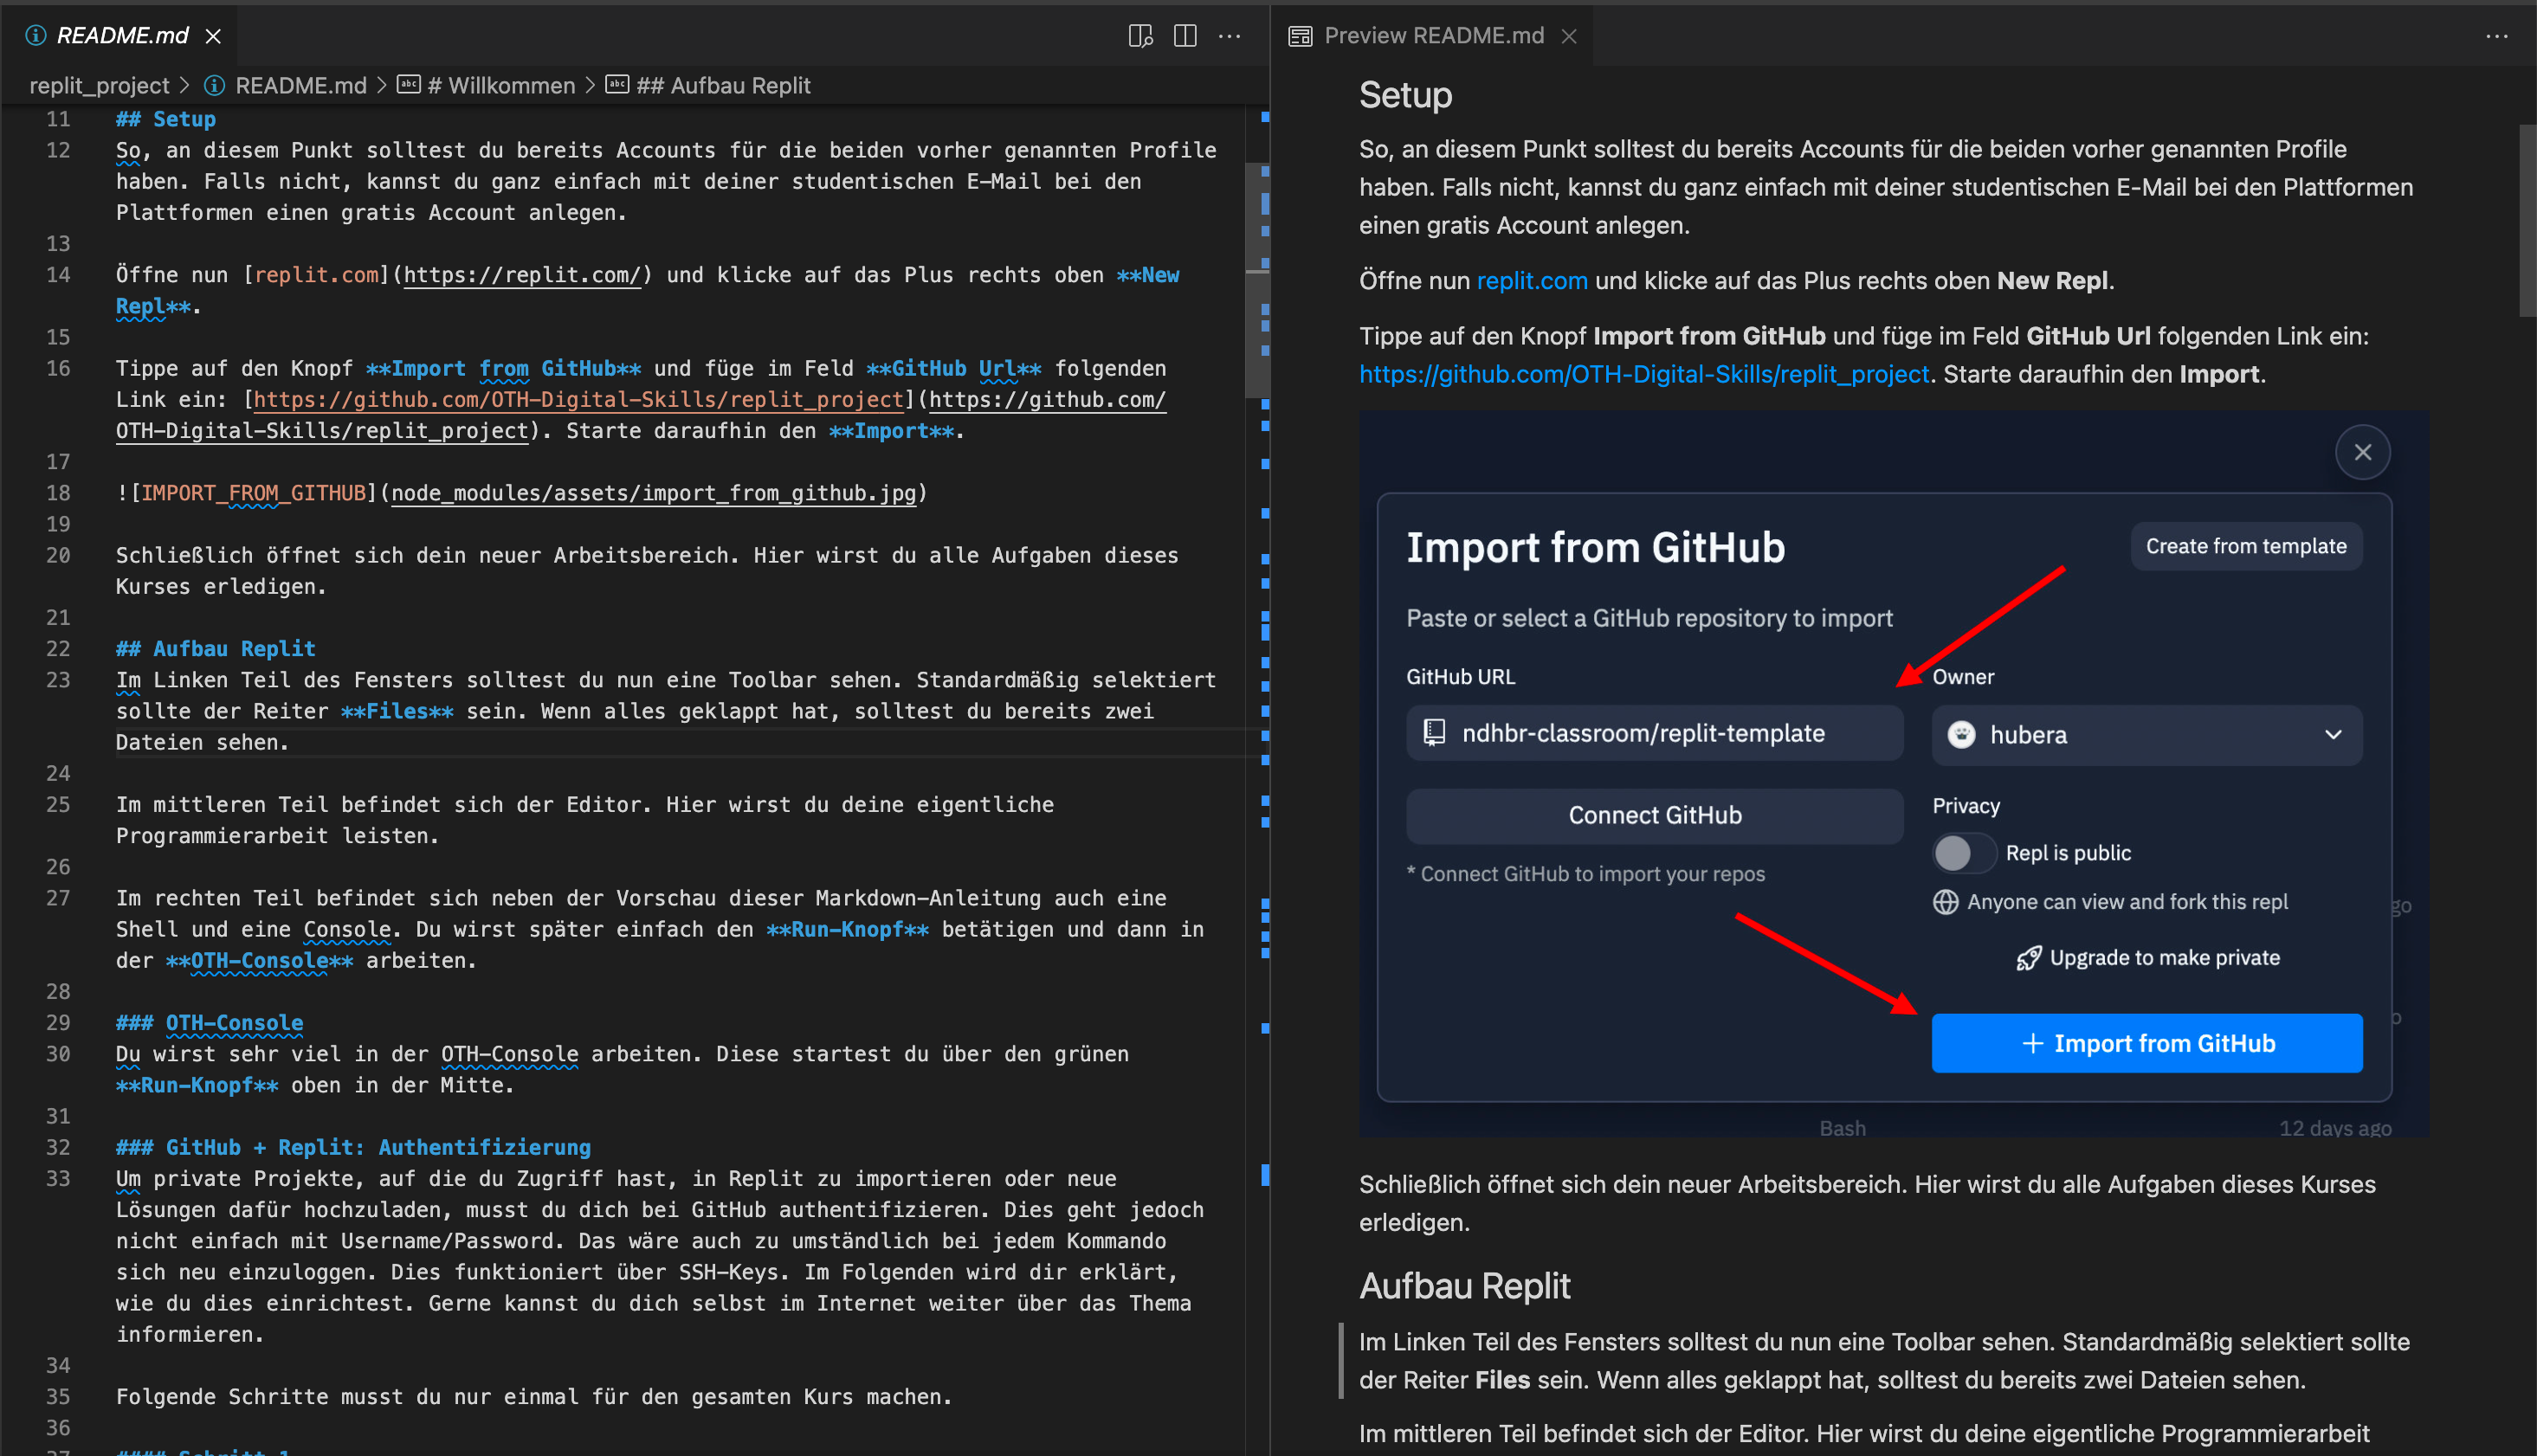
\includegraphics[width=\textwidth]{markdown}
    \caption{Erstellung eines Markdown-Dokuments}
    \bildquelle{Eigene Darstellung}
    \label{fig:markdown}
\end{figure}

\subsubsection{Replit als Online-Entwicklungsumgebung}
Der Programmierkurs soll für jeden Teilnehmer ohne komplizierte Installationen
durchführbar sein. Aus diesem Grund wurde die Entscheidung gefällt, eine
Online Entwicklungsumgebung einzusetzen.

Der Vorteil an Replit ist, dass man dem Studierenden durch ein
Vorlagenrepository alle nötigen Konfigurationen und Programme im Vorhinein
bereitstellen kann. Sobald ein sogenanntes \emph{Repl} (Bezeichnung für
ein Projekt in Replit) mit der erwähnten Vorlage erstellt wurde, kann der
Studierende ohne Installation geräteübergreifend online programmieren
\parencite{replit-import-from-github}. Der Teilnehmer muss daraufhin lediglich
auf den \glqq Run\grqq{}-Knopf drücken, welcher die später näher erläuterte
\emph{OTH-Console} startet und schließlich alle benötigten Abhängigkeiten
bereitstellt.

\subsubsection{GitHub Classroom als Abgabe- und Bewertungssystem}
GitHub Classroom eignet sich, für den Einsatz an der Hochschule, vor allem durch
seine Flexibilität und Einfachheit. Durch diese Flexibilität ist es möglich,
GitHub Classroom nur als eine austauschbare Komponente des Systems zu sehen.
Classroom übernimmt im System die Rolle des Aufgabenservers. Hier werden alle
Aufgabenvorlagen, sowie alle Versuche der Studierenden gespeichert und bewertet.

Sollte diese Komponente des Systems ausfallen, besteht weiterhin Replit als
Online-IDE, sowie Tutors mit den jeweiligen Anleitungen. Dadurch muss lediglich
ein adäquater Ersatz für GitHub Classroom gefunden und installiert werden.

% Konfiguration und Implementierung
\newpage
\section{Konfiguration und Implementierung}\label{konfiguration-u-impl}

% Tutors.dev
\subsection{Tutors als Aufgabensammlung}\label{tutors-als-aufgabensammlung}
Da der Programmierkurs nur ein Teil eines ganzen Modulkatalogs des Kurses
Digital Skills ist, übernehmen die Einrichtung Konfiguration von Tutors die
hierfür zuständigen wissenschaftlichen Mitarbeitenden des Zusatzstudiums.

Für die Einpflegung der Aufgaben werden lediglich Anleitungen sowie
jeweils dazugehörige Thumbnails (Vorschaubilder) benötigt. Die Anleitungen
werden, wie in Kapitel \ref{finale-architektur-tutors} genauer erläutert, im
standardisierten und weit verbreiteten Format Markdown verfasst.

Anleitungen können durch Markdown mit verhältnismäßig wenig Aufwand verfasst
werden und schließlich als \code{README.md}-Datei im Aufgaben-Repository
abgelegt werden. Dies hat den Vorteil, dass die Anleitung auch in der
Versionskontrolle der Aufgabe enthalten sind. Außerdem können GitHub und Replit
beim Klick auf die Aufgabe die Anleitung neben Tutors auch zusätzlich
formatiert anzeigen.

% GitHub Classroom
\subsection{GitHub Classroom}\label{github-classroom}
\subsubsection{Konfiguration}\label{classroom-konfiguration}
Für die Einrichtung wird eine GitHub Organisation erstellt. GitHub
Organisationen können von jedem GitHub-User erstellt werden und benötigen
lediglich einen Namen und eine Kontakt-E-Mail-Adresse
\parencite{github-organisation-erstellen}. Die Organisation dieses Kurses
beherbergt alle Aufgabenvorlagen, die später näher erläuterte Vorlage für
Replit, sowie alle Aufgabenrepositorys der Studierenden.

\subsubsection{Erste Aufgaben}\label{classroom-erste-aufgaben}
Nach der Erstellung der OTH-Organisation werden die Aufgabenvorlagen erstellt.
Aufgabenvorlagen sind in GitHub Classroom normale Repositorys, welche in GitHub
als Template markiert wurden. Sie beinhalten meist zusätzlich Unit-Tests, um den
Code darin zu prüfen.

Sobald die Organisation mit Aufgaben gefüllt ist, kann der
Classroom für den Kurs angelegt werden. Anfangs ist ein Classroom, wie die
Organisation auch, leer. Über die Oberfläche können neue Assignments
erstellt werden. Assignments sind Aufgaben, welche dem Studierenden zur
Verfügung stehen. Für jedes vorher angelegte Aufgabenrepository wird ein
Assignment erstellt. Bei der Erstellung gibt man verschiedene
Konfigurationsparameter an. Dazu gehört die Auswahl, ob eine Aufgabe von
Einzelpersonen oder einer Gruppe bearbeitet werden kann, oder ob die jeweiligen
Versuche für alle Studierenden oder nur für die Lehrenden sichtbar sind. Ferner
gibt es die Möglichkeit eine Deadline, sowie den Starter Code anzugeben. Für den
Starter Code wird in diesem Fall jeweils das Aufgabenrepository ausgewählt.
\parencite{github-assignment-erstellen}

\subsubsection{Tests und Benotung}\label{classroom-tests}
Im nächsten Schritt legt man die Benotung und das Feedback fest. Das Autograding
(die Benotung) geschieht über Kommandos in der Konsole. Im vorliegenden Fall
beinhaltet jedes Aufgabenrepository einen Ordner mit pytest-Tests. Pytest ist
eine Code-Test-Bibliothek für Python. Die Assignments wurden so konfiguriert,
dass GitHub nach jedem Push zum Repository des Studierenden die pytest-Tests
startet. Wenn alle Tests erfolgreich sind, erhält der Studierende eine
vorkonfigurierte Punktzahl. Durch Classroom ist es außerdem möglich, jedem
Test eine individuelle Punktzahl zuzuweisen. So kann man dem Schüler neben der
erfolgreichen Ausführung beispielsweise noch Bonuspunkte für das Berücksichtigen
von nicht geplanten Eingaben vergeben. \parencite{github-assignment-erstellen}

\newpage

% Replit
\subsection{Erstellung eines Replit-Starter-Templates}\label{replit-template}
\subsubsection{Template-Repository}\label{replit-template-repository}
% TODO: Quelle?
Projekte in Replit heißen \emph{Repls}. Ein Projekt ist in Replit ein
vollumfänglicher Arbeitsbereich, um neue oder bestehende Software zu entwickeln.
Neben einer Dateiübersicht, einem Texteditor und einer Konsole enthält der
Arbeitsbereich viele weitere Funktionen. Dazu zählt unter anderem eine
eingebaute Oberfläche für die Versionskontrolle Git, ein Quellcode-Debugger,
eine lokale Key-Value-Datenbank, private Umgebungsvariablen, sowie ein
spezieller Bereich für Unit-Tests.

Repls können auf Basis von bestehenden GitHub Repositorys erzeugt werden. Durch
den Import eines Repositorys, werden alle im Repository vorhandenen Dateien
in den neuen Arbeitsbereich kopiert. Diese Funktionalität ermöglicht das
Bereitstellen von Hilfsprogrammen und Dateien, die die Bearbeitung der
Kursaufgaben für den Teilnehmenden erleichtern.

Aus diesem Grund wurde ein öffentliches Repository in der vorher erstellten
GitHub Organisation angelegt. Dies ist das Template, welches später von den
Studierenden als Starter-Vorlage verwendet wird. Replit versteckt alle Dateien,
welche sich in einem Ordner namens \texttt{node\_modules} befinden.
Normalerweise wird der Ordner automatisch im Kontext mit externen Modulen der
JavaScript-Bibliothek Node.js verwendet \parencite{nodejs}. Das ist auch der
Grund, weshalb Replit diesen Ordner automatisch versteckt. Dieses Verhalten
nutzen wir, um Hilfsprogramme und Konfigurationen zu verstecken.

Studierende werden den ganzen Kurs in einem einzigen Repl absolvieren. Jede
Programmieraufgabe wird als Ordner im Repl Arbeitsbereich abgespeichert. Um die
Aufgaben herunterladen, prüfen und schließlich abgeben zu können, benötigt man
Git-Kenntnisse, sowie Erfahrungen mit Test-Frameworks, wie zum Beispiel pytest.
Im \texttt{node\_modules}-Ordner des Starter-Templates befinden sich diverse
Hilfsprogramme, welche den Studierenden bei der Einrichtung und Verwaltung der
Programmieraufgaben unterstützen.

\subsubsection{Hilfsprogramme (get, check, submit)}
\label{replit-template-wrapper-tools}
Die Kommandozeilen-Tools \texttt{get}, \texttt{check} und \texttt{submit} sind
\ac{bash} Skripte. Über den Konsolenbefehl \texttt{get <PROJEKT-REPOSITORY>}
kann der Studierende die Aufgabe in seinen Arbeitsbereich (Repl) laden. Das
Skript durchsucht die im Code definierte Organisation nach einem Repository mit
dem Namen und lädt es schließlich über den Befehl \code{git clone} in den
Arbeitsbereich.

Der Befehl \texttt{check <PROJEKT-REPOSITORY>} erlaubt es, die Aufgabe auf
Fehler überprüfen zu lassen. In jedem Aufgabenrepository befindet sich eine
\texttt{.language}-Datei, welche die für die Aufgabe verwendete
Programmiersprache enthält. Das \texttt{check}-Skript liest die
\texttt{.language}-Datei aus und entscheidet daraufhin, welche Befehle zum
Ausführen der Tests nötig sind. Python ist die vom Zusatzstudium Digital Skills
verwendete Programmiersprache. In diesem Fall installiert das Skript zuerst die
nötigen Abhängigkeiten mit

\begin{lstlisting}[style=Bash]
$ pip3 install pytest --quiet
\end{lstlisting}

Der Parameter \code{-{}-quiet} verhindert für den Teilnehmer unübersichtliche
Konsolenausgaben. Sobald das Testframework für Python installiert ist, führt das
Skript den Befehl \code{pytest} aus und startet somit die Ausführung der
Unit-Tests.

Schließlich pusht der Befehl \texttt{submit <PROJEKT-REPOSITORY>}
den Lösungsversuch in das GitHub Classroom Aufgabenrepository des
Kursteilnehmers. Dazu überprüft das Skript zuerst, ob es in der Zwischenzeit
Änderungen am Repository gab und lädt diese herunter. Anschließend erstellt
das Skript einen automatisierten Commit und lädt diesen in das Remote-Repository
in die GitHub-Organisation des Kurses hoch.

Damit die Skripte ordnerunabhängig ausgeführt werden können, werden
Konsolenaliase benötigt. Konsolenaliase können in einer Bash-Konsole
beispielsweise über das Anhängen folgender Zeile an die \texttt{.bashrc}-Datei
erstellt werden:

\begin{lstlisting}[style=Bash]
$ alias befehl="echo Hallo"
\end{lstlisting}

Bash ist eine Art \glqq Standard-Shell\grqq{} unter Linux und wird auch von
Replit als Konsole eingesetzt \parencite{bash}. Bei jeder neuen Konsolensitzung
wird dann der Alias aus der Datei eingelesen und angewendet. Die genannte Datei
befindet sich in der Regel im Benutzerverzeichnis, welches außerhalb des
Arbeitsbereiches in Replit liegt. Alle Änderungen außerhalb des Arbeitsbereiches
werden jedoch von Replit nach jeder Sitzung zurückgesetzt. Um dieses Problem zu
umgehen, wurde die nun folgende \emph{OTH-Console} entwickelt.

\subsubsection{OTH-Console}\label{replit-template-oth-console}
Sobald der Studierende in seinem Repl auf den Run-Knopf drückt, startet die
sogenannte OTH-Console in der Konsole. Dies ist eine neue
modifizierte Konsoleninstanz, welche alle für die Arbeit benötigten
Konfigurationen enthält.

Beim Start der OTH-Console beginnt die Ausführung des Einrichtungsskripts
\texttt{setup.py}, welches die benötigten Dateien in das Benutzerverzeichnis
schreibt.

Zuerst wird eine Konfigurationsdatei für Bash angelegt. In diese werden alle
benötigten Aliase (\texttt{get}, \texttt{submit}, \texttt{check} und
\texttt{github}) geschrieben. Außerdem wird GitHub, falls noch nicht vorhanden,
zu den sogenannten \emph{Known Hosts} im SSH-Ordner hinzugefügt. Der Vorteil
daran ist, dass der Studierende bei der ersten Verbindung mit GitHub (bspw. durch
den \texttt{get}-Befehl) keine SSH-Authentizitätsprüfung bestätigen muss
\parencite{ssh}. Als letztes wird in der Konfigurationsdatei noch das Aussehen
des \emph{Bash Promptes} festgelegt.

Im nächsten Schritt wird die passwortlose Authentifizierung mit GitHub
eingerichtet. Hierzu benötigt man ein SSH-Schlüssel-Paar, welches automatisch,
falls nicht vorhanden, durch das Einrichtungsskript erzeugt wird. Nach der
Erzeugung wird es neben dem SSH-Ordner auch in die Repl-Nutzer-Datenbank
geschrieben. Die Datebank ist ein simpler Key-Value-Speicher, welcher jeweils
pro Replit-Projekt existiert \parencite{replit-database}. Sobald der Studierende
Replit neu startet und das Benutzerverzeichnis gelöscht wurde, holt sich das
Einrichtungsskript die SSH-Keys aus der Datenbank und schreibt sie wieder
zurück in die jeweiligen Dateien. Dasselbe Verfahren wird ebenfalls für die
Konfiguration von Git angewandt. Git benötigt, um Commits zu pushen, einen 
Namen mit zugehöriger E-Mail-Adresse \parencite{git-config}. Diese Daten werden
zusammen mit den SSH-Keys in der Replit-Datenbank gespeichert.

Nach der Ausführung des Einrichtungsskripts, wird eine neue
Bash-Konsolen-Instanz, mit der gerade angelegten Konfigurationsdatei als
Parameter, gestartet.

\subsubsection{SSH-Keys}\label{replit-template-ssh-keys}
Um das vorher generierte SSH-Schlüsselpaar für die Authentifizierung gegen
GitHub zu verwenden, muss der öffentliche Schlüssel noch zu dem GitHub-Profil
des Studierenden hinzugefügt werden. Hierfür enthält das Starter-Template ein
weiteres Programm auf Basis von Python, welches mit dem Befehl \texttt{github}
in der OTH-Console ausgeführt werden kann. Dieses weitere Tool lädt den im
SSH-Ordner gespeicherten öffentlichen Schlüssel und gibt ihn zusammen mit einem
Link zum Hinzufügen von SSH-Keys in GitHub aus.

Des Weiteren überprüft das Programm, ob Git bereits konfiguriert ist. Um Commits
zu erstellen, benötigt Git wie vorher bereits erwähnt einen Namen sowie eine
dazugehörige E-Mail-Adresse. Sind die benötigten Werte nicht in der
Replit-Datenbank vorhanden, fragt das Programm den Nutzenden nach dem Namen und
der studentischen E-Mail-Adresse. Nach gültiger Eingabe der Daten werden diese
Werte in der nutzerspezifischen Replit-Datenbank des Arbeitsbereiches
hinterlegt. Damit Git die Werte übernehmen kann, werden sie, wie beim
Einrichtungsskript auch, in eine dafür vorgesehene Git-Konfigurationsdatei
geschrieben.

% Studie
\newpage
\section{Studie: Test an fachfremden Studierenden}\label{studie}
\subsection{Allgemein}
In einer Studie sollen Fehler und schwierig gestaltete Stellen der
Programmierplattform gefunden und analysiert werden. Damit die Studie möglichst
realitätsnah ist, fällt die Wahl hierbei auf eine Feldstudie mit fachfremden
Studierenden. \parencite{feldstudie}

Nach Vollendung der Tests sollen Schwachstellen und Lücken der
Programmieraufgaben (Anleitungen, Fehlerbeschreibungen, Aufbau, Schwierigkeit,
...) gefunden, behoben und für zukünftige Aufgaben berücksichtigt werden.
\parencite{studie-testkonzept}

\subsection{Methode}
Um für jeden Durchlauf gleiche Testbedingungen sicherstellen zu können, wird ein
Testkonzept ausgearbeitet. Bei jeder Durchführung wird sich auf die Regeln
und den Ablauf des Testkonzepts bezogen.

Das Testkonzept legt im Grunde die Metadaten der Studie fest. Neben der
Zielsetzung, der Zielgruppe und der Dauer des Tests wird in dem Konzept auch die
Methodik festgelegt.

\subsubsection{Teilnehmende}
Die Zielgruppe der Studie lässt sich durch wenige Parameter definieren. Sie
ist äquivalent zur Zielgruppe des Zusatzstudiums Digital Skills. Gesucht sind
folglich Studierende, welche keine Studiengänge der Fakultät Informatik und
Mathematik belegen. Durch diese Einschränkung qualifiziert man sich für die
Teilnahme am Zusatzstudium Digital Skills und dadurch implizit auch für die
Anteilnahme an der folgenden Studie.

Um eine gleichmäßig verteilte Stichprobenmenge zu erhalten, werden mindestens
fünf Testpersonen aus fünf unterschiedlichen Studiengängen für die Durchführung
benötigt. Wie in Tabelle \ref{table:studie-teilnehmende} absolut dargestellt,
ist das Geschlechterverhältnis mit zwei Drittel männlichen Teilnehmern sehr
ausgeglichen. In folgender Tabelle ist neben dem Geschlecht auch das jeweilige
Alter der Testpersonen, sowie der Studiengang und das Semester visualisiert.

\begin{table}[H]
\renewcommand*{\arraystretch}{1.6}
\centering
\begin{tabular}{|l|l|l|l|}
\hline
\textbf{Geschlecht} & \textbf{Alter} & \textbf{Studiengang}                      & \textbf{Semester} \\ \hline
Weiblich            & 22             & Betriebswirtschaftslehre (B.A.)           & 5                 \\ \hline
Weiblich            & 21             & Bauingenieurwesen (B.Eng.)                & 5                 \\ \hline
Weiblich            & 22             & Psychologie (M.Sc.)                       & 3                 \\ \hline
Männlich            & 23             & Brauwesen und Getränketechnologie (M.Sc.) & 1                 \\ \hline
Männlich            & 23             & Regenerative Energietechnik (B.Eng.)     & 6                 \\ \hline
\end{tabular}
\caption{Studienteilnehmer:innen}

\label{table:studie-teilnehmende}
\end{table}

\subsubsection{Ablauf des Tests}
Die Studienbefragungen finden zwischen dem 11. Februar 2022 und dem 6. März
2022 statt. Die Tests werden in Form eines Interviews online über eine Software
für Videokonferenzen durchgeführt.

Am Anfang wird vom Beobachter der Studie, Andreas Huber, das Zusatzstudium
Digital Skills anhand eines einseitigen Infodokuments vorgestellt.

Danach wird dem Teilnehmer die folgende Agenda vorgetragen und anschließend
werden der Person vier Fragen gestellt. Die Fragen müssen jeweils mit Schulnoten
von 1 bis 6 beantwortet werden. Sechs bedeutet hier immer eine gänzliche
negative Neigung, während eins einer völligen Zusage entspricht. Die restlichen
Noten bilden wie gewohnt lineare Zwischenwerte.

Nachdem die Fragen von der teilnehmenden Person beantwortet wurden, muss diese
die Bildschirmübertragung starten. Währenddessen notiert der Beobachter die
Ergebnisse der Fragen in eine vorher angelegte Tabelle.

Der Teilnehmer wird anschließend darauf hingewiesen, dass die Studie der
Think-Aloud-Methodik folgt. Die Think-Aloud-Methode ist eine Forschungsmethode,
bei der der Testteilnehmer darum gebeten wird, seine Gedanken laut
auszusprechen. Mit dieser Methode können mögliche Aufhänger und Probleme in den
Anleitungen der Aufgaben leichter gefunden werden. Der Beobachter des Tests
schreibt alle Anomalien kategorisiert nach Fortschritt und Teilnehmer des Tests
auf. \parencite{think-aloud}

Aufkommende Fragen können vom Beobachter beantwortet werden. Sollte eine Frage
bzw. Aufgabe unlösbar erscheinen, gibt es am Ende jeder Aufgabe ein
Lösungsvorschlag. Dieser sollte jedoch nur aufgeklappt werden, wenn keine
realistische Chance der selbstständigen Lösung des Problems besteht.

Als Nächstes werden die im folgenden Kapitel \ref{studie-materialien}
erläuterten Aufgaben durch den Testteilnehmer bearbeitet. Während der
Bearbeitung wird die dafür benötigte Zeit durch den Beobachter mit einer
Stoppuhr gestoppt.

Abschließend kann der Studierende die Bildschirmübertragung wieder beenden und
sich auf das Nachgespräch konzentrieren. Hierbei werden dem Teilnehmer noch
fünf weitere Fragen gestellt. Die Fragen müssen wie vorher in Schulnoten von 1
bis 6 beantwortet werden. Die Ergebnisse der Fragen werden wie gewohnt vom
Beobachter notiert und in die vorher erwähnte Datentabelle eingetragen.

Als grober Leitfaden wird die Dauer von 30 bis 60 Minuten festgelegt, dies soll
jedoch kein hartes Zeitlimit darstellen. Der Test soll möglichst unabhängig
ablaufen und kann bei möglichen Unverständnissen auch deutlich länger dauern.
Gemäß einer Feldstudie darf das Ergebnis der Studie nicht durch eine mögliche 
Manipulation, wie beispielsweise durch eine zeitliche Barriere, verfälscht
werden.

Auf eine Entschädigung der Teilnehmenden wird aufgrund mangelnder Budgets
verzichtet. Alle Teilnehmenden absolvieren die Studie freiwillig.

\subsubsection{Materialien}\label{studie-materialien}
\paragraph{Fragen}
Folgende Fragen werden den Teilnehmenden vor Beginn der Bearbeitung gestellt:

\begin{itemize}
    \item Hast du schon einmal erwägt eine Programmierausbildung anzustreben?
    (1: will ich definitiv noch machen; 6: noch nie) \textbf{[PRE1]}
    \item Hast du schon einmal programmiert? (1: ständig; 6: noch nie)
    \textbf{[PRE2]}
    \item Wie fit fühlst du dich am PC? (1: sehr fit; 6: gar nicht)
    \textbf{[PRE3]}
    \item Würde für dich das Zusatzstudium Digital Skills in Frage kommen?
    (1: unbedingt; 6: auf keinen Fall) \textbf{[PRE4]}
\end{itemize}

Nach Bearbeitung der Aufgaben müssen die Studierenden noch folgende fünf
Fragen beantworten:

\begin{itemize}
    \item Wie schwer kam dir die Einrichtung, bis zu dem Punkt, an dem du die
    erste Aufgabe heruntergeladen hast, vor? (1: sehr leicht; 6: sehr schwer)
    \textbf{[PAST1]}
    \item Hattest du Schwierigkeiten mit Aufgabe 1? (1: nein, keine; 6: zu
    komplex) \textbf{[PAST2]}
    \item Hattest du Schwierigkeiten mit Aufgabe 2? (1: nein, keine; 6: zu
    komplex) \textbf{[PAST3]}
    \item Hast du verstanden was du in den Aufgaben genau gemacht hast? (1: ja
    vollkommen; 6: nein, gar nicht) \textbf{[PAST4]}
    \item Würdest du nach Abschluss des Tests deine Meinung zur Frage am
    Interesse eines Zusatzstudiums für Digital Skills ändern? (1: unbedingt;
    6: auf keinen Fall) \textbf{[PAST5]}
\end{itemize}

Alle aufgezeigten Fragen wurden durch den Beobachter und Initiator der Studie,
Andreas Huber, selbst erfunden. Die in eckigen Klammern stehenden Bezeichnungen
dienen zur Identifikation der jeweiligen Fragen für die später folgende
Auswertung.

\paragraph{Aufgaben}
Der Test besteht aus vier für die Studie vereinfachten Aufgaben. Die erste
Aufgabe beschäftigt sich lediglich mit der Einrichtung des Arbeitsplatzes in
Replit und GitHub-Classroom. Die Studierenden sind dazu aufgefordert, das in 
Kapitel \ref{replit-template} besprochene Replit-Template zu klonen und in 
Replit einzurichten. Dazu gehört das Hinzufügen des SSH-Keys zu GitHub, sowie
das Herunterladen der ersten Aufgabe.

Die zweite Aufgabe ist eine Programmieraufgabe mit der Sprache Python. Es
handelt sich hierbei um eine vereinfachte Version der später in produktiv
eingesetzten Aufgabe \glqq Lab 4: Hello\grqq{}. Die bereits gegebene Vorlage der
Aufgabe fragt den Nutzenden nach seinem Namen. Nach der Eingabe schließt sich
das Programm wieder. Die Aufgabe des Teilnehmenden ist es nun den Namen in
folgendem Format wieder auszugeben: \code{Hallo, mein Name ist <NAME>}. Der
Platzhalter \code{<NAME>} soll dabei durch den vorher abgefragten Namen ersetzt
werden. Diese Aufgabe kann der Teilnehmer mit einer einzigen Codezeile lösen.
Die Ausgabe der Lösung sieht dann so aus:

\begin{lstlisting}[style=Bash]
$ python main.py
Wie ist dein Name? Andreas
Hallo, mein Name ist Andreas!
\end{lstlisting}

Der ausgegebene Name ist wie vorher beschrieben flexibel und abhängig von der
Eingabe des Nutzers.

Die dritte Aufgabe ist ebenfalls eine Programmieraufgabe mit der Sprache Python.
In dieser Aufgabe geht es um die erste Verwendung einer \texttt{for}-Schleife.
Am Anfang der Anleitung wird sehr ausführlich erklärt, was eine
\texttt{for}-Schleife ist, weshalb man sie braucht und wie man sie anwendet.
Danach wird die Aufgabenstellung erklärt, welche ähnlich zur zweiten Aufgabe
ist. Dieses Mal wird der Nutzer nach Start des Programms nicht nur nach seinem
Namen gefragt, sondern auch nach der Anzahl, wie oft der Name ausgegeben werden
soll. Wie auch in der vorherigen Aufgabe schließt sich standardmäßig das
Python-Skript gleich wieder. Der Testteilnehmer muss nun eine Schleife
programmieren, dass der Name mit der aktuellen Zählvariable n-mal ausgegeben
wird. Der Name und die Anzahl an Ausgaben wird wieder per Funktion als Parameter
übergeben. Die Ausgabe in der Konsole soll wie folgt aussehen:

\begin{lstlisting}[style=Bash]
$ python main.py
Wie ist dein Name? Andreas
Wie oft soll der Name ausgegeben werden? 5
Andreas 0
Andreas 1
Andreas 2
Andreas 3
Andreas 4
\end{lstlisting}

Falls die Aufgaben reibungslos funktioniert haben, kann der Studierende
die Herausforderung einer optionalen Bonusaufgabe annehmen. Um diese
Bonusaufgabe zu lösen, muss der Teilnehmer die vorherige Aufgabe modifizieren,
sodass die Ausgabe in der Konsole wie folgt aussieht:

\begin{lstlisting}[style=Bash]
$ python main.py
Wie ist dein Name? Andreas
Wie oft soll der Name ausgegeben werden? 5
Andreas 1
Andreas 2
Andreas 3
Andreas 4
Andreas 5
\end{lstlisting}

Der Unterschied hier ist die Nummerierung. Im Standardfall zählt das Programm
von 0 bis n - 1. Um die Bonusaufgabe zu bewältigen, muss das Programm von 1 bis
n zählen.

Die vierte und letzte Aufgabe beschäftigt sich mit der Generierung von
Text-Pyramiden, welche der ursprünglichen Version des Videospiels Super Mario
Bros.\copyright\footnote{Super Mario Bros.\copyright ist eine geschützte Marke
der Nintendo Co., Ltd.} entsprechen sollen. Der Nutzer wird beim Start des
Programms nach der gewünschten Größe bzw. Höhe der Pyramide. Nach Eingabe eines
gültigen  Werts liefert das Skript, ausgegeben mit Raute-Zeichen, die linke
Seite einer klassischen Super Mario Pyramide. Die Ausgabe der gelösten Aufgabe
sieht beispielhaft so aus:

\begin{lstlisting}[style=Bash]
$ python main.py
Höhe: -1
Höhe: 0
Höhe: 6
     #
    ##
   ###
  ####
 #####
######
\end{lstlisting}

Das Beispiel zeigt neben der Pyramide auch, dass das Skript ungültige
Größenangaben erkennen und ignorieren soll. Aufgrund der erhöhten Schwierigkeit
dieser Aufgabe wurde entschieden, die letzte Aufgabe für die Feldstudie zu
verwerfen.

\paragraph{Test-Classroom}
Für die Vorbereitung der Interviews wird eine neue GitHub-Organisation, sowie
ein neuer GitHub-Classroom angelegt. Sowohl das Replit-Template als auch die im
vorherigen Kapitel beschriebenen Aufgaben werden als Template-Repositories in
der Test-Organisation abgelegt.

Für die Aufgaben werden mithilfe des Test-Frameworks pytest Benotungstests
programmiert und in GitHub-Classroom konfiguriert. Jede gelöste Aufgabe belohnt
den Studienteilnehmenden pauschal mit 10 Punkten.

Neben den Programmieraufgaben werden auch ausführliche Anleitungen mit Bilder
geschrieben. Nach der Erstellung von Vorschaubildern können diese in der,
auch später produktiv genutzten, Plattform Tutors hochgeladen werden. Die
Studienteilnehmer:innen erhalten zu Beginn des Probelaufs einen Link zur
Übersicht der benötigten Anleitungen in Tutors.

\newpage
\subsection{Deskriptive Ergebnisse}
Nach Verarbeitung der Ergebnisse der Fragen können nun die einzelnen Resultate
analysiert und interpretiert werden. Die folgende Tabelle \ref{table:studie}
enthält in Spalte 1 die Identifikationsbezeichnung der Frage. Spalte 2 und
3 beinhaltet den Durchschnitt und die dazugehörige \ac{sd}. Die vierte, fünfte
und sechste Spalte enthalten den Medianwert, das Minimum und schließlich das
Maximum der Antworten.

\begin{table}[H]
    \renewcommand*{\arraystretch}{1.6}
    \centering
    \begin{tabular}{|l|l|l|l|l|l|} 
    \hline
    \diagbox{\textbf{Fragen}}{\textbf{Ergebnisse}} & \textbf{Durchschnitt } & \textbf{SD} & \textbf{Median } & \textbf{Min.} & \textbf{Max.}  \\ 
    \hline
    \textbf{Alter }                                & 22.200                 & 0.837       & 22.000           & 21            & 23             \\ 
    \hline
    \textbf{PRE1 }                                 & 3.600                  & 2.300       & 3.000            & 1             & 6              \\ 
    \hline
    \textbf{PRE2 }                                 & 2.600                  & 1.670       & 3.000            & 1             & 5              \\ 
    \hline
    \textbf{PRE3 }                                 & 2.600                  & 0.894       & 2.000            & 2             & 4              \\ 
    \hline
    \textbf{PRE4 }                                 & 2.600                  & 1.820       & 2.000            & 1             & 5              \\ 
    \hline
    \textbf{PAST1 }                                & 2.600                  & 1.520       & 2.000            & 1             & 5              \\ 
    \hline
    \textbf{PAST2 }                                & 3.200                  & 1.300       & 4.000            & 1             & 4              \\ 
    \hline
    \textbf{PAST3 }                                & 3.800                  & 1.790       & 5.000            & 1             & 5              \\ 
    \hline
    \textbf{PAST4 }                                & 2.200                  & 1.100       & 3.000            & 1             & 3              \\ 
    \hline
    \textbf{PAST5 }                                & 3.800                  & 2.170       & 3.000            & 1             & 6              \\
    \hline
    \end{tabular}

    \caption{Auswertung der Studienergebnisse}
    \label{table:studie}
\end{table}

% Alter
Wie man der Alterszeile entnehmen kann, sind alle Teilnehmenden im Schnitt 22
Jahre alt. Dieses Ergebnis lässt sich vor allem aus der Anforderung schließen,
dass alle Teilnehmenden immatrikulierte Studierende sein müssen.

% PRE1, PRE2
Die Ergebnisse der Fragen PRE1 und PRE2 deuten darauf hin, dass die Interessen
der Teilnehmer sehr gemischt sind. Der Bereich zwischen Minimum und Maximum ist
in beiden Fragen sehr hoch. Dies verdeutlicht, dass es sowohl Teilnehmende gibt,
die bereits ständig mit Programmieren zu tun haben, als auch welche, die noch
absolut keine Berührungen mit der Materie hatten.

% PRE3
Das Wohlbefinden am Computer wurde mit der Frage PRE3 abgefragt. Ein
Interpretationsversuch der Minima und Maxima ist, dass die Teilnehmenden aus
Angst später Fehler zu machen niemals die Note 1 vergeben haben. Damit ist diese
Frage auch die einzige mit Schulnoten zu bewertende Frage, welche in der Umfrage
keine Note 1 als Minimum enthält.

% PRE4 - PAST5
Die Frage PRE4 bezieht sich auf das Interesse an einem Zusatzstudium für
Digital Skills. Der Durchschnitt der Antworten auf diese Frage liegt bei 2,600,
der Median noch besser bei 2,000. Das heißt, dass die Mehrheit der Testpersonen,
vor der Bearbeitung der Aufgaben, einer Teilnahme an einem solchen Zusatzstudium
nicht abgeneigt wären. Nach der Absolvierung der Programmieraufgaben werden die 
Teilnehmer erneut nach ihrer Meinung bzw. einer Änderung dieser Einschätzung
gefragt (Frage: PAST5). Hier wird anhand des Durchschnitts, sowie des Medians
eine deutliche negative Tendenz ersichtlich. Durch die hohe Standardabweichung
bei der Frage PAST5, kann man nicht auf eine vollständige Abneigung der
Studierenden schließen. Trotzdem kann die negative Tendenz des Interesses auf zu
schwere oder dürftig erklärte Aufgaben hindeuten. Ein weiterer
Interpretationsversuch ist, dass die Studierenden nach der Präsentation des 
Zusatzstudiums andere Vorstellungen zu den Modulen hatten.

% PAST1, PAST2, PAST3
Die Fragen PAST1, PAST2 und PAST3 beziehen sich jeweils auf das
Schwierigkeitsempfinden der Studierenden gegenüber den drei Programmieraufgaben.
Die erste Programmieraufgabe ist in diesem Fall die Einrichtungsaufgabe des
Arbeitsbereiches. Mit dem Design der Aufgaben wird versucht die Schwierigkeit
mit jeder Aufgabe zu steigern. Die Durchschnitte der Umfrage bestätigen den
Erfolg eines linearen Schwierigkeitsanstiegs. Während PAST1 einen Durchschnitt
von 2,600 aufweist, scheint die Schwierigkeit bei der ersten
Python-Programmieraufgabe (PAST2) mit einem Durchschnittswert von 3,200 deutlich
höher zu liegen. Erneut gesteigert hat sich das Schwierigkeitsempfinden mit der
dritten Aufgabe (PAST3) auf einen Durchschnittswert von 3,800. Die Differenz der
Durchschnitte beträgt bei beiden Anstiegen genau 0,800 Notenpunkte.

% PAST4
Das allgemeine Verständnis der Aufgaben wird mit der Frage PAST4 abgefragt. Für
diese Frage wurde die 3 als Maximalnote aufgezeichnet. Der Durchschnitt liegt
wiederum bei 2,200 Notenpunkte und ist somit im positiven Bereich.

\section{Zusammenfassung und Ausblick}\label{zusammenfassung-u-ausblick}
\newpage

% Römische Nummerierung
\pagenumbering{roman}
\setcounter{page}{3}

% Abbildungsverzeichnis
\listoffigures
\newpage

% Literaturliste soll im Inhaltsverzeichnis auftauchen
\phantomsection
\addcontentsline{toc}{section}{Quellenverzeichnis}
% Literaturverzeichnis anzeigen
\renewcommand\refname{Quellenverzeichnis}
\printbibliography
% \bibliography{assets/literatur}
\newpage

\end{document}